%%%%%%%%%%%%%%%%%%%%%%%%%%%%%%%%%%%%%%%%%%%%%%%%%%%%%%%%%%%%%%%%%%%%%%
%%        Copyright (c) 2016 Carsten Wulff Software, Norway
%% %%%%%%%%%%%%%%%%%%%%%%%%%%%%%%%%%%%%%%%%%%%%%%%%%%%%%%%%%%%%%%%%%%%
%% Created       : wulff at 2016-11-5
%% %%%%%%%%%%%%%%%%%%%%%%%%%%%%%%%%%%%%%%%%%%%%%%%%%%%%%%%%%%%%%%%%%%%
%%   This program is free software: you can redistribute it and/or modify
%%   it under the terms of the GNU General Public License as published by
%%   the Free Software Foundation, either version 3 of the License, or
%%   (at your option) any later version.
%%
%%   This program is distributed in the hope that it will be useful,
%%   but WITHOUT ANY WARRANTY; without even the implied warranty of
%%   MERCHANTABILITY or FITNESS FOR A PARTICULAR PURPOSE.  See the
%%   GNU General Public License for more details.
%%
%%   You should have received a copy of the GNU General Public License
%%   along with this program.  If not, see <http://www.gnu.org/licenses/>.
%%%%%%%%%%%%%%%%%%%%%%%%%%%%%%%%%%%%%%%%%%%%%%%%%%%%%%%%%%%%%%%%%%%%%%



\documentclass[journal,12pt,draftclsnofoot,onecolumn,letterpaper]{IEEEtran}

\usepackage[final]{graphicx}
\usepackage{wrapfig}

\ifCLASSINFOpdf
\graphicspath{{../../pdf/}}
\DeclareGraphicsExtensions{.pdf}
\else
\graphicspath{{../../eps/}}
\DeclareGraphicsExtensions{.eps}
\fi

\usepackage{setspace}

\linespread{1.9}

\usepackage[nomarkers]{endfloat}
\renewcommand{\efloatseparator}{\smallskip}
\let\MYoriglatexcaption\caption
\renewcommand{\caption}[2][\relax]{\MYoriglatexcaption[#2]{#2}}

\newcommand{\myfigwidth}{3.5in}
\newcommand{\myfigwidthb}{\linewidth}

%%%%%%%%%%%%%%%%%%%%%%%%%%%%%%%%%%%%%%%%%%%%%%%%%%%%%%%%%%%%%%%%%%%%%%
%% Copyright (c) 2016 Carsten Wulff Software, Norway
%% %%%%%%%%%%%%%%%%%%%%%%%%%%%%%%%%%%%%%%%%%%%%%%%%%%%%%%%%%%%%%%%%%%%
%% Created       : wulff at 2016-11-5
%% %%%%%%%%%%%%%%%%%%%%%%%%%%%%%%%%%%%%%%%%%%%%%%%%%%%%%%%%%%%%%%%%%%%
%% This program is free software: you can redistribute it and/or modify
%% it under the terms of the GNU General Public License as published by
%% the Free Software Foundation, either version 3 of the License, or
%% (at your option) any later version.
%%
%% This program is distributed in the hope that it will be useful,
%% but WITHOUT ANY WARRANTY; without even the implied warranty of
%% MERCHANTABILITY or FITNESS FOR A PARTICULAR PURPOSE.  See the
%% GNU General Public License for more details.
%%
%% You should have received a copy of the GNU General Public License
%% along with this program.  If not, see <http://www.gnu.org/licenses/>.
%%%%%%%%%%%%%%%%%%%%%%%%%%%%%%%%%%%%%%%%%%%%%%%%%%%%%%%%%%%%%%%%%%%%%%


%\usepackage{placeins}
\usepackage{upgreek}
\usepackage{amssymb,amsmath}
\usepackage{cite}
\usepackage{verbatim}
\usepackage{listings}
\usepackage{xcolor}
\usepackage{flafter}
\usepackage{booktabs}
\usepackage{url}
\usepackage{ textcomp }

\hyphenation{op-tical net-works semi-conduc-tor}


% -JSON styel

%\definecolor{darkGreen}{rgb}{0,0.2097,0}
%\newcommand{\myfigwidth}{\linewidth}
%\newcommand{\myfigwidtha}{\linewidth}
%\newcommand{\myfigwidthl}{\textwidth}
%\newcommand{\myfigwidthc}{0.6\linewidth}


\newcommand{\myfigwidtha}{3.3in}
\newcommand{\myfigwidthl}{7in}
\newcommand{\myfigwidthc}{2in}
%\newcommand{\myfigwidthe}{3.2in}
%\newcommand{\myfigwidthb}{5in}

\newcommand{\myfigname}{fig_}
\newcommand{\reg}[2]{{\figurename} \ref{#1}(#2)}
\newcommand{\req}[1]{{\figurename} \ref{#1}}
%\newcommand{\myeqname}{eq:}
%\newcommand{\req}[1]{(\ref{\myeqname#1})}

\definecolor{armygreen}{rgb}{0, 0.5, 0}
\newcommand{\missing}[1]{{ #1}}
\newcommand{\edit}[1]{{ #1}}
\newcommand{\secedit}[1]{{ #1}}
\newcommand{\deleted}[1]{{ #1}}
\newcommand{\moved}[1]{{ #1}}

%\newcommand{\missing}[1]{{\color{red} #1}}
%\newcommand{\edit}[1]{{\color{red} #1}}
%\newcommand{\secedit}[1]{{\color{armygreen} #1}}
%\newcommand{\deleted}[1]{{\color{violet} #1}}
%\newcommand{\moved}[1]{{\color{blue} #1}}

\newcommand{\SD}{Sigma-Delta }
\newcommand{\eqn}[1]{
  \begin{equation}
    #1
  \end{equation}}

\newcommand\JSONnumbervaluestyle{\color{blue}}
\newcommand\JSONstringvaluestyle{\color{red}}

\newif\ifcolonfoundonthisline

\makeatletter

\lstdefinestyle{json}
{
  showstringspaces    = false,
  keywords            = {false,true},
  alsoletter          = 0123456789.,
  morestring          = [s]{"}{"},
  stringstyle         = \ifcolonfoundonthisline\JSONstringvaluestyle\fi,
  MoreSelectCharTable =%
  \lst@DefSaveDef{`:}\colon@json{\processColon@json},
  basicstyle          = \fontsize{7}{7}\ttfamily,
  keywordstyle        = \fontsize{7}{7}\ttfamily\bfseries,
}

% flip the switch if a colon is found in Pmode
\newcommand\processColon@json{%
  \colon@json%
  \ifnum\lst@mode=\lst@Pmode%
  \global\colonfoundonthislinetrue%
  \fi
}

\lst@AddToHook{Output}{%
  \ifcolonfoundonthisline%
  \ifnum\lst@mode=\lst@Pmode%
  \def\lst@thestyle{\JSONnumbervaluestyle}%
  \fi
  \fi
  % override by keyword style if a keyword is detected!
  \lsthk@DetectKeywords%
}

% reset the switch at the end of line
\lst@AddToHook{EOL}%
{\global\colonfoundonthislinefalse}

\makeatother

% \lstset{  basicstyle=\tiny}

% \lstset{
% basicstyle=\fontsize{11}{13}\selectfont\ttfamily
% }


\lstset{language=Java}


\lstdefinestyle{paperBashStyle}{
  language=bash,
  stepnumber=1,
  numbersep=10pt,
  basicstyle=\footnotesize\ttfamily,
  tabsize=4,
  showspaces=false,
  showstringspaces=false
}



\begin{document}

\bibliographystyle{IEEEtran}


% Version history:





\title{A Paper framework}
%
\author{Carsten~Wulff, \textit{Member, IEEE} }

\maketitle

\begin{abstract}
This is a framework for writing papers, I've used it for JSSC publications. Feel free to use it for what you want.

Carsten Wulff (Corresponding author), carste@wulff.no

\end{abstract}
\begin{IEEEkeywords}
latex
\end{IEEEkeywords}

\section{Introduction} \label{introduction}


\IEEEPARstart{W}{riting} beautiful papers is can be split into two, typesetting and content. I can't help you on the content, but this framework is something that's been developed over the years to do the typesetting with latex.

\section{Getting Started}

\begin{lstlisting}[frame=single,style=paperBashStyle]
mkdir <whatever your paper is called>
cd <whatever your paper is called>
git clone https://github.com/wulffern/paper
make -f paper/Makefile install
make all
\end{lstlisting}

\section{Directories}

The "tex" directory contain the source files. It also will contain a couple examples on how to compile figures in tikz and circuitikz.


\section{Figures}

I would recommend that you make your figures using tikz. Yes, it takes time, but it's the only
way I've found to make beautiful pictures. Like the methodology used in \cite{Wulff17} where I published \cite{ciccreator16}

\begin{figure}[tb]
\centerline{\includegraphics[width=\myfigwidth]{fig_process}}
\caption{\secedit{Design methodology}}
\label{fig_cic}
\end{figure}

Or the circuit tikz pictures that can be made, which was used in the same paper
\begin{figure}[tb]
\centerline{\includegraphics[width=\myfigwidth]{fig_comparator}}
\caption{\edit{Strong-arm comparator with kick-back
  compensation. Transistors without numbers are unit size, while
  transistors with numbers are parallel combinations of unit transistors.}}
\label{fig_comp}
\end{figure}



\bibliography{../bib/wulff_compiledsar.bib}


\begin{wrapfigure}{l}{0.2\textwidth}
\centerline{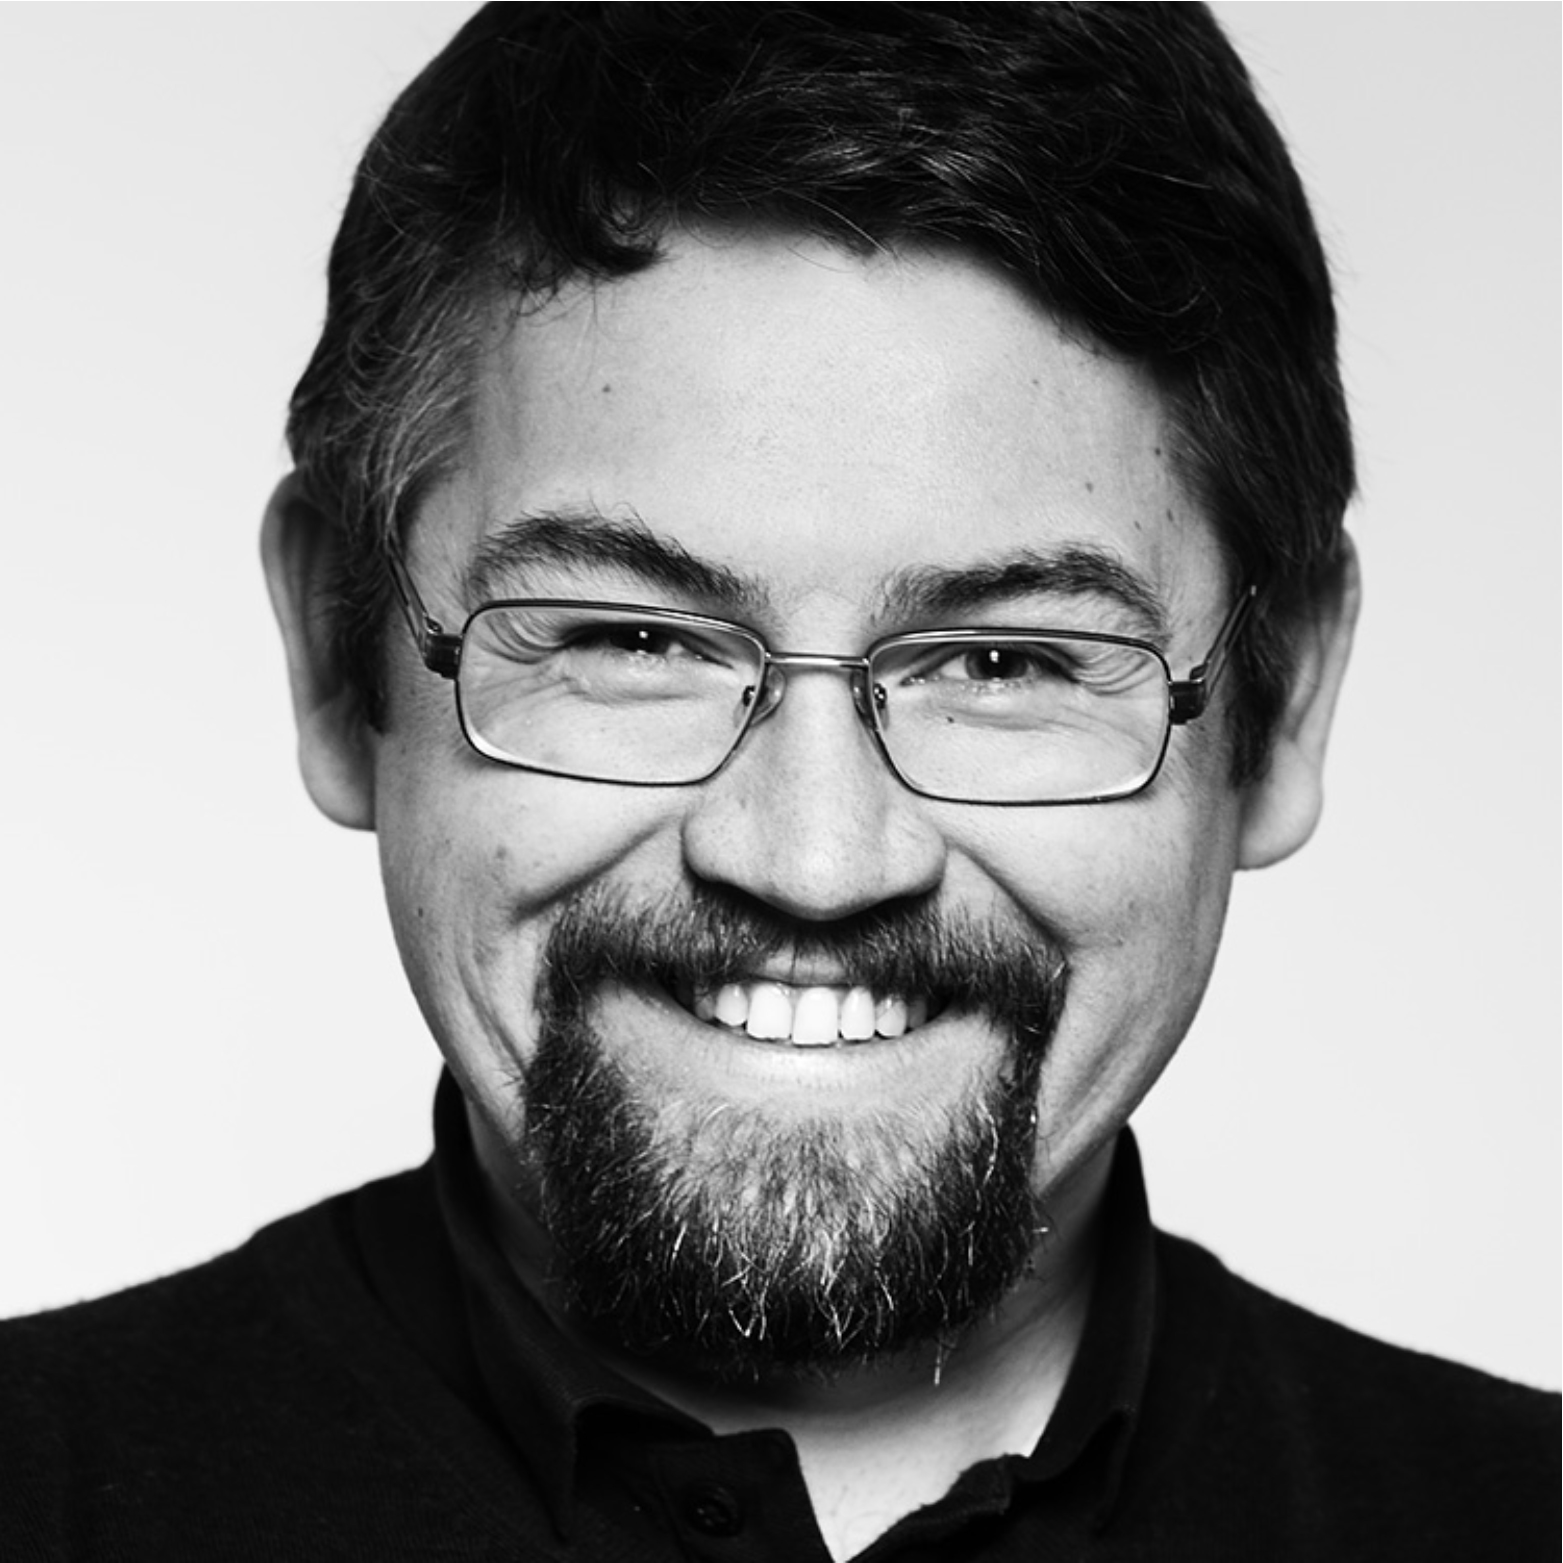
\includegraphics[width=30mm]{wulff} }
\end{wrapfigure}

 \textbf{Carsten Wulff}
received the M.Sc. and Ph.D. degrees in
electrical engineering from the Department of Electronics and Telecommunication, Norwegian University of Science and Technology (NTNU),
in 2002 and 2008, respectively.
During his Ph.D. work at NTNU, he worked on open-loop sigma-delta
modulators and analog-to-digital converters in nanoscale CMOS
technologies. In 2006-2007, he was a Visiting Researcher with the
Department of Electrical and Computer Engineering, University of
Toronto, Toronto, ON, Canada. He is currently the Group Manager for the
Wireless Group at Nordic Semiconductor ASA, Trondheim, Norway and a
Post Doctoral fellow at NTNU. His
present research interests includes analog and mixed-signal CMOS
design, design of high-efficiency analog-to-digital converters and
low-power wireless transceivers. He is the developer of Custom IC
Compiler, a general purpose integrated circuit compiler.

\end{document}
